\chapter{Cosmological Evolution}

In this chapter we briefly describe the evolution of the Universe. For more comprehensive lectures see e.g. \textcite{Ref:Weinberg}, \textcite{2002col.luc..cosmology} or \textcite{2010deto.book.....A}. We begin with basic equations for the evolution and apply them to cosmological scales. We describe different epoch in history of the Universe and also introduce number of cosmic distances often used to put observational constraints on dark energy. We show some fundamental issues with the simplest models -- horizon problem, missing (dark) matter and accelerated expansion of the Universe -- and arrive to concordance \LCDM\ model. We describe background evolution and formation of structures in \LCDM\ model and introduce some basic observables. At the end of the chapter we outline some issues with the cosmological constant and offer some basic alternative in modified gravity models.

\section{Background evolution}
\todo{cite cosmological principle}
Standard cosmological model is based on the \textit{cosmological principle}, first clearly formulated in \textcite{1687pnpm.book.....N}. The cosmological principle states that the Universe is homogeneous and isotropic on sufficiently large scales (beyond those traced by the large-scale structure of the distribution of galaxies). The cosmic microwave background (CMB) observations strongly support this statement as photons from different parts of the Universe are coming with almost identical temperatures. This isotropy, however, does not imply homogeneity. The \textit{Copernican Principle} states that the observer is not in a special place or time. With the observed isotropy the Copernican Principle implies the Cosmological Principle. The observed inhomogeneities and irregularities on local scales come from gravitational instability and do not violate these principles.
%%%%%%%%%%%%%%%%%%%%%%%
% Friedmann equations
%%%%%%%%%%%%%%%%%%%%%%%
\subsection{Friedmann equations}
The homogeneous and isotropic space-time is described by Friedmann-Lema\^{i}tre-Robertson-Walker (FLRW) metric given by
\eq{
    \label{eq:flrw}
    \dd s^2=g_\uv\dd x^\mu \dd x^\nu=-\dd t^2+a^2(t)\left[\frac{\dd r^2}{1-Kr^2} + r^2\left(\dd\theta^2+\sin^2\theta\dd\phi^2 \right) \right]\,,
}
where $g_{\mu\nu}$ is a metric tensor, $a(t)$ is a scale factor with cosmic time $t$ and $K=+1,-1,0$ is a curvature that corresponds to closed, open, and flat geometries. The scale factor can be arbitrary rescaled and we adopt the common normalization $a_0=1$. We can also transform metric \eqref{eq:flrw} to a more convenient form by setting $r=\sin\chi\ (K=+1),r=\chi\ (K=0)$, and $r=\sinh\chi\ (K=-1)$. The FLRW metric is then given by
\eq{
    \label{eq:flrw_chi}
    \dd s^2=-\dd t^2+a^2(t)\left[\dd \chi^2 + f_K^2(\chi)\left(\dd\theta^2+\sin^2\theta\dd\phi^2 \right)\right]\,,
}
where
\eq{
    f_K(\chi)=
    \begin{cases}
        \sin\chi & (K=+1)\,, \\
        \chi & (K=0)\,, \\
        \sinh\chi & (K=-1)\,.
    \end{cases}
}
By allowing taking the limit $K\to0$ we can rewrite $f_K(\chi)$ in a unified way
\eq{
    \label{eq:f_K}
    f_K(\chi)=\frac{1}{\sqrt{-K}}\sinh{(\sqrt{-K}\chi)}\,.
}
In addition to the cosmic time $t$, we also introduce the conformal time $\eta$ defined by
\eq{
    \eta\equiv\int{a^{-1}\dd t}\,.
}
The dynamical equations of motion in the expanding Universe can be derived from the Einstein equations resulting in the Friedmann equations
\eq{
    \label{eq:Friedmann}
    H^2 &= \frac{8\pi G}{3}\rho - \frac{K}{a^2}+\frac{\Lambda}{3}\,, \\
    \label{eq:Friedmann_2}
    \frac{\ddot a}{a} &= -\frac{4\pi G}{3}(\rho + 3p)+\frac{\Lambda}{3}\,,\\
    \label{eq:Friedmann-continuity}
    \dot\rho &= -3H(\rho+p)\,,
}
\todo{comment $\Lambda$}

where the overdot denotes a time derivative with respect to $t$, $H\equiv\dot a/a$ is the Hubble parameter, $\Lambda$ the cosmological constant (more details at the end of this chapter), $\rho(t)$ is energy-density and $p$ pressure. We will be also using the conformal Hubble quantity
\eq{
    \mathcal{H}\equiv\frac{1}{a}\frac{\dd a}{\dd\eta}=Ha\,.
}
These three equations are not independent and we need to also specify the equation of state, $\rho=\rho(p,t)$. The first equation is usually also written in the form
\eq{
    \Omega_m+\Omega_\gamma+\Omega_K+\Omega_\Lambda=1\,,
}
where
\eq{
    \label{eq:omega}
    \Omega_m\equiv\frac{8\pi G\rho_m}{3H^2}\,,\hspace{3pt}
    \Omega_\gamma\equiv\frac{8\pi G\rho_\gamma}{3H^2}\,,\hspace{3pt}
    \Omega_K\equiv-\frac{K}{a^2H^2}\,,\hspace{3pt}
    \Omega_\Lambda\equiv\frac{\Lambda}{3H^2}
}

Most matter species in the Universe can be described by a simple equation of state
\eq{
    p=w\rho\,,
}
where $w$ is constant. This lead to the following solutions in flat universe
\eq{
    \rho\propto a^{-3(1+w)}\,,\hspace{6pt}a\propto (t-t_i)^{2/(3(1+w)))}\,,
}
where $t_i$ is an integration constant. Relativistic matter has the equation of state $w=1/3$ and the cosmic evolution during the radiation-dominated epoch is given by $w\propto a^{-4}$ and $a\propto(t-t_i)^{1/2}$. Non-relativistic matter has negligible pressure $(w=0)$ and the evolution during the matter- dominated era is given by $w\propto a^{-3}$ and $a\propto(t-t_i)^{2/3}$.

The accelerated expansion of the Universe $(\ddot a>0)$ without the cosmological constant is possible only for $w<-1/3$ (see Friedman equation \eqref{eq:Friedmann_2}), i.e. negative pressure. Note that in Newtonian gravity there is no such equivalent. The pressure is related to a force associated with a local potential that depends on the position in space but in homogeneous and isotropic universe there is no such potential.

When $w=-1$, the energy-density $\rho$ is constant and corresponds to the cosmological constant. This energy-density connected to the cosmological constant is
\eq{
    \rho_\Lambda=\frac{\Lambda}{8\pi G}\,.
}
With constant energy-density the Friedmann equations lead to an exponential expansion $a\propto\exp{Ht}$.

%%%%%%%%%%%%%%%%%%%%%%%
% Hubble`s law
%%%%%%%%%%%%%%%%%%%%%%%
\subsection{Hubble`s law}
During the 1920s astronomers Slipher and Hubble found that the observed wavelength $\lambda_o$ of absorption lines of distant galaxies is larger than the wavelength $\lambda$ in the rest frame \parencite{1929PNAS...15..168H}. This is due to the fact that the wavelength is stretched in proportion to the scale factor in an expanding Universe. The redshift $z$ is defined as
\eq{
    z\equiv\frac{\lambda_0}{\lambda} - 1=a^{-1}-1\,.
}
In an expanding Universe a physical distance $r$ from an observer (at the origin) to an object is given by $r=a(t)x$, where $x$ denotes the comoving distance. For objects which are motionless with respect to the Hubble flow the comoving distance remains constant. Taking the time derivative of $r$ we obtain
\eq{
    v_H\equiv\dot r=Hr+a\dot x
}
Because of the cosmic expansion, more distant objects are moving faster from us with velocity $v_H$. On the other hand, the peculiar velocity $v_p\equiv a\dot x$ describes the movement of an object with respect to the local Hubble flow. For small peculiar velocities and near objects $(z\ll1)$ we obtain
\eq{
    v\sim H_0r\,,
}
which is the law Hubble reported in 1929 by plotting the recessional velocity $v$ versus the distance $r$. His measurements were noisy but the current measurements give the Hubble constant the value \parencite{planck_cosm}
\eq{
    H_0=(67.4\pm0.5)\rm{\ km\ s}^{-1}\rm{Mpc}^{-1}
}

%%%%%%%%%%%%%%%%%%%%%%%
% Cosmic distances
%%%%%%%%%%%%%%%%%%%%%%%
\subsection{Cosmic distances}
\todo{Move closer to cosmo. observ.? This would fix prime notation changes.}

In the expanding Universe there are many ways to specify the distance between two points due to the constantly changing distances and the fact that observers look back in time as they look out in distance.
\subsubsection{Comoving distance}
The light traveling along the $\chi$ direction satisfies the geodesic equation $\dd s^2=-\dd t^2+a^2(t)\dd \chi^2=0$. The light emitted at the time $t=t_1$ with $\chi=\chi_1$ (redshift $z$) reaches an observer at time$t=t_0$ with $\chi=0$ (redshift $z=0$). Integrating the geodesic equation
\eq{
    \label{eq:d_c}
    d_c\equiv\chi_1=\int_0^{\chi_1}\dd\chi=-\int_{t_0}^{t_1}\frac{\dd t}{a(t)}=\frac{1}{H_0}\int_0^z\frac{\dd\tilde z}{E(\tilde z)}\,,
}
where
\eq{
    E(z)\equiv H(z)/H_0=\sqrt{\Omega_{\gamma,0}(z+1)^4+\Omega_{m,0}(z+1)^3+\Omega_{K,0}(z+1)^2+\Omega_{\Lambda,0}}\,.
}
If we expand $E(z)$ around $z=0$ we can write the cosmic distance as
\eq{
    d_c=\frac{1}{H_0}z-\frac{E'(0)}{2H_0}z^2+\frac{2E'(0)^2-E''(0)}{6H_0}z^3+\mathcal{O}(z^4)\,,
}
where a prime represents a derivative with respect to $z$.
\subsubsection{Luminosity distance}
The luminosity distance $d_L$ is used in supernovae observations in order to link the supernova luminosity with the expansion rate of the Universe. It is defined by
\eq{
    d_L^2\equiv\frac{L_s}{4\pi F}\,,
}
where $L_s$ is the absolute bolometric (i.e., integrated over all frequencies) luminosity of a source and $F$ is the observed bolometric flux. The flux is defined by $F=L_0/S$, where $L_0$ is the observed luminosity and $S=4\pi f_K^2(\chi)$ is the area of a sphere at $z=0$.

The absolute luminosity is defined as energy emitted per unit time interval, $L=\Delta E/\Delta t$. The energy of a photon is inversely proportional to its wavelength, $E\propto\lambda^{-1}\propto 1+z$, which is stretching in an expanding universe. Also the time between arrival of two photons is proportional to the wavelength, $\Delta t\propto\lambda\propto(1+z)^{-1}$. The ratio $L_s/L_0$ is then
\eq{
    \frac{L_s}{L_0}=\frac{\Delta E_1}{\Delta E_0}\frac{\Delta t_0}{\Delta t_1}=(1+z)^2\,,
}
and the luminosity distance is
\eq{
    d_L=f_K(\chi)(1+z)\,.
}
Using definition \(f_K\) \eqref{eq:f_K} and comoving distance \eqref{eq:d_c} we can express $d_L$ as
\eq{
    \label{eq:luminosity}
    d_L=\frac{1+z}{H_0\sqrt{\Omega_{K,0}}}\sinh{\left(\sqrt{\Omega_{K,0}}\int_0^z{\frac{\dd\tilde z}{E(\tilde z)}}\right)}\,.
}
For small $z$ we can once again expand the expression and get
\eq{
    d_L=\frac{1}{H_0}z-\frac{E'(0)-2}{2H_0}z^2+\frac{2E'(0)^2-3E'(0)-E''(0)+\Omega_{K,0}}{6H_0}z^3+\mathcal{O}(z^4)\,.
}
\subsubsection{Angular diameter distance}
The angular diameter distance $d_A$ is defined as
\eq{
    d_A\equiv\frac{\Delta x}{\Delta\theta}\,,
}
where $\Delta\theta$ is the angle that subtends an object of actual size$\Delta x$ orthogonal to the line of sight. Whenever we look at objects of known size such as CMB anisotropies or BAO scale we use this distance.

The observer measures the size $\Delta x$ along the surface of a sphere with radius $\chi$ and from metric \eqref{eq:flrw_chi} follows
\eq{
    \Delta x=a(t)f_K(\chi)\Delta\theta\,.
}
The angular diameter distance is then
\eq{
    \label{eq:angular}
    d_A=a(t)f_K(\chi)=\frac{1}{1+z}\frac{1}{H_0\sqrt{\Omega_{K,0}}}\sinh{\left(\sqrt{\Omega_{K,0}}\int_0^z{\frac{\dd\tilde z}{E(\tilde z)}}\right)}\,.
}
Comparing angular diameter distance \eqref{eq:angular} and luminosity distance \eqref{eq:luminosity} we can see that they have a following relation
\eq{
    d_A=\frac{d_L}{(1+z)^2}\,.
}
\subsubsection{Degeneracy of the distance measurements}
We can se that up to the first order all the distances are the same and reduce to the Euclidean distance and that the Hubble`s law holds. With the increasing redshift the Hubble`s law dos not hold exactly and also different distances behave differently. This can be used to measure different properties of the Universe.

As the distances depend on the cosmological parameters through the integral $\int_0^z{\dd\tilde z/E(\tilde z)}$ and through $\Omega_K$ we can measure only those parameters contained in $E(z)$. Moreover, if we had distance measurements only around one particular redshift $z$ any combination of parameters that would produce similar $E(z)$ would be equally acceptable. This degeneracy can be broken by combination of measurements across different redshifts or by using other cosmological probes.

%%%%%%%%%%%%%%%%%%%%%%%
% Formation and evolution of LSS
%%%%%%%%%%%%%%%%%%%%%%%
\section{Formation and evolution of LSS}
So far we have considered only equations for smooth, homogeneous and isotropic background. In order to describe the real Universe with its rich structures we must employ perturbation theory for cosmological equations.
\subsection{Newtonian gauge}
We will consider first order (linear) perturbations of the metric:
\eq{
    g_{\mu\nu}=g_{\mu\nu}^{(0)}+\delta g_{\mu\nu}\,,
}
where $g_{\mu\nu}^{(0)}$ is the FLRW metric \eqref{eq:flrw} and all the entries in the perturbed metric $\delta g_{\mu\nu}$ have to be small with respect to the background metric. The general perturbed metric can be written as
\eq{
    \delta g_{\mu\nu}=a^2(\eta)
    \begin{pmatrix}
        -2\Psi & w_i \\
        w_i & 2\Phi\delta_{ij}+h_{ij} \\
    \end{pmatrix}\,,
}
where $\Psi(t,x)$ and $\Phi(t,x)$ are spatial scalars, $w_i(t,x)$ is 3-vector, and $h_{ij}(t,x)$ is a traceless 3-tensor. We have a freedom to choose coordinates in which we will describe the equations of motion -- we can choose our \textit{gauge}. We wish to keep our background metric $g_{\mu\nu}^{(0)}$ the same (i.e. FLRW) and only change $\delta g_{\mu\nu}$. Note that unlike ordinary coordinate transformations a gauge transformation (although expressed as a change of coordinates) does not link different observers in the same spacetime but it links two different spacetimes seen by the same observer. For a detailed discussion of gauge choices, see e.g. \textcite{PhysRevD.40.1804}, \textcite{10.1143/PTPS.78.1} or \textcite{PhysRevD.22.1882}.

We will choose to attach the observers to the points in the unperturbed frame, the so called \textit{Newtonian} or \textit{longitudinal} or \textit{shear-free} gauge. In this case the observer will detect a velocity field of particles falling into the clumps of matter and will measure a gravitational potential. We can impose up to four conditions on the metric, which corresponds to the four gauge coordinate transformations. The final perturbed metric is:
\eq{
    \label{eq:flrw_pert}
    \dd s^2=a^2(\eta)\left[-(1+2\Psi)\dd\eta^2+(1+2\Phi)\delta_{ij}\dd x^i\dd x^j\right]\,.
}
\subsection{Linear perturbations}
We now decompose the Einstein tensor and the energy-momentum tensor into background and perturbed parts. The background cosmological evolution is obtained by solving the zero-th order Einstein equations and is given by the Friedmann equations. The first order equations are given by the perturbation of the Einstein tensor, i.e. by perturbed metric \eqref{eq:flrw_pert}, and by the perturbed energy-momentum tensor $T_\uv$. The energy-momentum tensor for a single perfect fluid is given by
\eq{
    T_\uv=\left(\rho+p\right)u_\mu u_\nu + pg_\uv\,,
}
where the four-velocity $u^\mu$ is up to the first order
\eq{
    u^\mu\equiv\dddd{x^\mu}{\tau}=\left[\frac{1}{a}(1-\Psi),\frac{v^i}{a} \right]\,,
}
where $\tau$ is the proper time and $v^i=\dd x^i/\dd\eta$ is the matter peculiar velocity with respect to the general expansion. We also assume that the perturbed fluid remains perfect fluid. We will use the following notation
\eq{
    \delta &\equiv\frac{\delta\rho}{\bar{\rho}}\equiv\frac{\rho-\bar{\rho}}{\bar{\rho}}\,,\\
    \theta &\equiv\nabla\cdot v\,,
}
where $\delta$ is the density contrast, the bar represents a mean value (spatial average) and $\theta$ is the velocity divergence. The first order equations are (for details see e.g. \cite{2002col.luc..cosmology} or \cite{10.1143/PTPS.78.1})
\eq{
    \label{eq:lin_1}
    3\mathcal{H}(\mathcal{H}\Psi-\Phi') + \nabla^2\Phi &= -4\pi G\bar\rho a^2 \delta\,,\\
    \label{eq:lin_2}
    \nabla^2(\Phi' - \mathcal{H}\Psi) &= 4\pi G\bar\rho a^2(1+w)\theta\,,\\
    \label{eq:lin_3}
    \Psi &=-\Phi\,,\\
    \label{eq:lin_4}
    \Phi''+2\mathcal{H}\Phi'-\mathcal{H}\Psi-(\mathcal{H}^2+2\mathcal{H}')\Psi &=-4\pi G\bar\rho a^2c^2_s\delta\,,
}
where the prime now denotes the derivative with respect to the conformal time $\eta$. Sound velocity $c_s$ is defined as
\eq{
    c_s^2\equiv\frac{\delta p}{\delta\rho}=\dddd p\rho = \frac{\dot p}{\dot\rho}\,,
}
where the last equality are valid only in the FLRW metric at background level. Conservation of the energy-momentum tensor leads to the perturbed continuity equation
\eq{
    \delta'+3\mathcal{H}(c_s^2-w)\delta=-(1+w)(\theta+3\Psi')\,,
    \label{eq:lin_5}
}
which reduces for non-relativistic matter to
\eq{
    \delta'=-\theta-3\Phi'\,.
}
Another equation coming from the conservation of the energy-momentum tensor is
\eq{
    \theta'+\left[\mathcal{H}(1-3w)+\frac{w'}{1+w}\right]\theta=-\nabla^2\left(\frac{c_s^2}{1+w}\delta + \Psi \right)\,,
    \label{eq:lin_6}
}
which reduces for non-relativistic matter to
\eq{
    \theta'+\mathcal{H}\theta=-\nabla^2\Psi-\nabla^2(c_s^2\delta)\,,
}
which is a relativistic analog of the Euler equation.


We will now transform all the equations to the Fourier space. The Fourier transformation is (up to non-relevant pre-factors)
\eq{
    f(\bm{x})=\int e^{i\bm{k\cdot x}}\hat{f}(\bm k)\dd^3k\,,
}
where $\bm k$ is a wavenumber with modulus $k$ and hat represents quantities in Fourier space. If there is no danger of misunderstanding we will drop the hat in the following. Since we are dealing with linear equations the different modes are not coupled and we can solve the equation for each $k$ independently.
 From equations \eqref{eq:lin_1}---\eqref{eq:lin_4}, \eqref{eq:lin_5} and \eqref{eq:lin_6} we will obtain the following equations in Fourier space:
\eq{
    \label{eq:lin_k_1}
    k^2\Phi + 3\mathcal{H}(\Phi'-\mathcal{H}\Psi) &= 4\pi G\bar\rho a^2 \delta\,,\\
    \label{eq:lin_k_2}
    k^2(\Phi' - \mathcal{H}\Psi) &= -4\pi G\bar\rho a^2(1+w)\theta\,,\\
    \label{eq:lin_k_3}
    \Psi &=-\Phi\,,\\
    \label{eq:lin_k_4}
    \Phi''+2\mathcal{H}\Phi'-\mathcal{H}\Psi-(\mathcal{H}^2+2\mathcal{H}')\Psi &=-4\pi G\bar\rho a^2c^2_s\delta\,,\\
    \label{eq:lin_k_5}
    \delta'+3\mathcal{H}(c_s^2-w)\delta &= -(1+w)(\theta+3\Psi')\,,\\
    \label{eq:lin_k_6}
    \theta'+\left[\mathcal{H}(1-3w)+\frac{w'}{1+w}\right]\theta &= k^2\left(\frac{c_s^2}{1+w}\delta + \Psi \right)\,,
}
where now $\theta=i\bm{k\cdot  v}$. Note that these six equations are not independent and $w$ and $c_s^2$ are arbitrary functions of time.
\subsubsection{Super-horizon scales}
In the large-scale limit $k\ll\mathcal{H}$, i.e. when the physical wavelength $\lambda_p=2\pi a/k$ of perturbations is much larger than the Hubble radius $H^{-1}$, and with the barotropic fluid, i.e. when the pressure depends only on the energy density, and with the constant $w$, we have $c_s^2=w$ and we can get an equation for $\Phi$
\eq{
    \Phi''+3\mathcal{H}(1+c_s^2)\Phi'=0\,.
}
The growing / dominant solution for $c_s^2>-1$ is $\Phi=\rm{const}$ from which follows
\eq{
    3\mathcal{H}^2\Phi=4\pi G\bar\rho a^2\delta\,.
}
Using the Friedmann equation we get $\delta=\Phi$, i.e. $\delta$ remains constant at large scales whenever $c_s^2=w$.
\subsubsection{Sub-horizon scales}
In the small-scale limit $k\gg\mathcal{H}$ we can get for a pressureless fluid $(w=0)$ with a small sound speed $c_s^2\ll1$ the Poisson equation
\eq{
    \label{eq:poisson_lin}
    k^2\Phi=4\pi G\bar\rho a^2\delta\,,
}
and the energy conservation equation
\eq{
    \delta' &= \theta \\
    \theta' &= -\mathcal{H}\theta + c_s^2k^2\delta-k^2\Phi\,.
}
These equations lead to
\eq{
    \delta'' +\mathcal{H}\delta' +\left(c_s^2k^2 + \frac32\mathcal{H}^2 \right)\delta=0\,.
}
Perturbations on small scales with $(c_s^2k^2-\frac32\mathcal{H})>0$ do not grow but undergo damped oscillations. These are perturbations with physcial wavelength smaller than the Jeans length
\eq{
    \lambda_J=c_s\sqrt\frac{\pi}{G\bar\rho}\,.
}
For the photons and baryons before the decoupling epoch we have $c_S=c/sqrt3$ and the Jeans length is comparable to the Hubble radius $H^{-1}$ and the growth of perturbations is prevented on all scales smaller than that. For a small sound speed $c_sl\ll\mathcal{H}$ the perturbations grow freely (gravitational instability). The resulting equation for a single pressureless fluid becomes
\eq{
    \label{eq:lin_evol_m}
    \delta''+\mathcal{H}\delta'-\frac32\mathcal{H}^2\delta=0\,.
}
The growing solution during the matter dominated era is $\delta\propto a\propto t^{2/3}$ and the gravitational potential remains constant during this epoch.

%%%%%%%%%%%%%%%%%%%%%%%
% Growth function
%%%%%%%%%%%%%%%%%%%%%%%
\subsubsection{Growth function and rate}
In linear perturbation theory the gravitational evolution of fluctuations is separable into time-dependent and spatially-dependent (or wavenumber-dependent) parts, i.e.
\eq{
    \delta(a)=\delta_0D(a)\,,
}
where $\delta_0$ is present overdensity and the growth function $D$ is normalized as $D(a=1)\equiv1$. The logarithmic change of growth function is the growth rate $f$
\eq{
    \label{eq:grw_rate}
    f\equiv\dddd{\ln D}{\ln a}\,.
}
 A very good approximation of a solution to density evolution \eqref{eq:lin_evol_m} is
\eq{
    f\approx|\Omega_m(a)|^\gamma\,,
}
where $\gamma\approx0.55-0.6$ depends only weakly on cosmological parameters \parencite{1980_Peebles}.

%%%%%%%%%%%%%%%%%%%%%%%
% Photon propagation
%%%%%%%%%%%%%%%%%%%%%%%
\subsection{Photon propagation}
The above equations describe the evolution of matter density perturbations. Now we will focus on the propagation of light in this perturbed Universe. The photon momentum is defined via $k^\mu=\dd x^\mu/\dd\lambda_s$, where $\lambda_s$ is an affine parameter. The equations for the propagation are then
\eq{
    k_\mu k^\mu &= 0\,,\\
    \label{eq:p_geo}
    \dddd{k^\mu}{\lambda_s}+\Gamma^\mu_{\alpha\beta}k^\alpha k^\beta &= 0\,.
}
We will split the momentum vector into a background and a perturbed value $k^\mu=\bar k^\mu+\delta k^\mu$. The photon moves in the unperturbed metric along the direction $r$ so that $\dd\eta=\dd r$. At the background level we can integrate the photon path \eqref{eq:p_geo} to get $\bar k^0\propto a^{-2}$ and therefore the photon frequency $\nu\equiv\dd t/\dd\Lambda_s=a\bar k^0\propto a^{-1}$ as expected. The equations for the perturbed part $\delta k$ are \parencite[for details see e.g. ][]{2010deto.book.....A}
\eq{
    \label{eq:SW_0}
    \dddd{(\delta k^0/k^0)}{\eta} &= -\left(\partpart{\Phi}{\eta}+\partpart{\Psi}{\eta}+2\partpart{\Psi}{r}\right)\,,\\
    \label{eq:WL_0}
    \frac{\dd^2x^i}{\dd\lambda_s^2}+2\mathcal{H}\dddd{\eta}{\lambda_s}\dddd{x^i}{\lambda_s} &= \left(\partpart{\Phi}{x^i}-\partpart{\Psi}{x^i}\right)\,,
}
where the two directions $x^1$ and $x^2$ are orthogonal to the propagation direction $r$.
\subsubsection{The Sachs--Wolfe effect}
The time part of the geodesic equations \eqref{eq:SW_0} describes changes in the frequency (redshift) of photons passing through changing gravitational potentials. Integrating the equation along the light-ray null path from the time of emission $e$ to the time of observation $o$ gives us
\eq{
    \left.\frac{\delta k^0}{k^0}\right\rvert_e^o=-2\left.\Psi\right\rvert_e^o-\int_{e}^{o}{\left(\partpart\Phi\eta-\partpart\Psi\eta\right)\dd\eta}\,,
}
where vertical bars represents change of quantities between $e$ and $o$. The first effect is referred to as the \textit{Sachs--Wolfe effect} and depends on the difference between the potential at emission and at observation. The second effect is called the \textit{integrated Sachs--Wolfe effect} and depends on the line-of-sight integral of $\Phi-\Psi$.
\subsubsection{Weak lensing}
The spatial part of the geodesic equations \eqref{eq:WL_0} can be written for $i=1,2$ as
\eq{
    \frac{\dd^2x^i}{\dd r^2}=\partpart{\psi}{x^i}\,,
}
where the lensing potential $\psi\equiv\Phi-\Psi$. For small displacements we can put $x^i=r\theta^i$. Integrated the above equation gives us
\eq{
    \theta^i=\theta^i_0+\int_0^r\dd r'\left(1-\frac{r'}{r}\right)\partpart{\psi(r'\theta_0^1,r'\theta_0^2,r')}{x^i}\,.
}
Two light rays separated by a small angle  $\Delta\theta^i$ on the source plane at $r=r_s$ are connected to the the observation plane at $r=0$ by the symmetric transformation matrix
\eq{
    A_{ij}\equiv\partpart{\theta^i_s}{\theta^j_o}=\delta_{ij}+D_{ij}\,,
}
where the distortion tensor
\eq{
    D_{ij}=\int_0^{r_s}\dd r'\left(1-\frac{r'}{r_s}\right)r'\frac{\partial^2\psi}{\partial x^i\partial x^j}=
    \begin{pmatrix}
        -\kappa-\gamma_1 & -\gamma_2 \\
        -\gamma_2 & -\kappa + \gamma_1
    \end{pmatrix}
    \,.
}
The convergence $\kappa$ describes the magnification of the source image and the two components of the shear field $\gamma_1,\gamma_2$ describe the distortion of the source image.
%%%%%%%%%%%%%%%%%%%%%%%
% Non-linear cosmological perturbations
%%%%%%%%%%%%%%%%%%%%%%%
\subsection{Non-linear cosmological perturbations}
So far we have described linear gravitational processes which are essential for cosmolgy as a whole and approximate methods we are exploring. However, as we will compare our results with full \nbodysim s, which can deal with the full non-linear dynamics, we will mention here a regime that lies between the linear perturbation theory and the full non-linear gravitational interactions.

One step further from linear order are the second-order perturbations. In this approximation one no longer neglect terms like divergence of the velocity field and the resulting equations are much more complicated than the linear order \textcite[see e.g.][]{2004astro.ph.12025T,10.1093/mnras/264.2.375,2010deto.book.....A}. We will mention here only the simplest result for a spherical perturbation in Einstein--de Sitter universe with initial Gaussian perturbations \textcite{1980_Peebles}:
\eq{
    \delta &= \delta^{(1)}+\delta^{(2)}\,,\\
    \delta^{(1)} &= \delta_0(\mb x)D_L(a)\,,\\
    \delta^{(2)} &= \delta_0^2(\mb x)D_2(a)\,,\\
    D_2 &= \frac{17}{21}D_L^2\,.
}
In general, solutions of higher order perturbations has to be found numerically and they are computationally similarly expensive as \nbodysim s described later in this work.

Another non-linear effet of cosmological importance is the spherical collapse. The model of spherical collapse describes non-linear evolution of a spherical perturbation in an otherwise smooth expanding background. The equations and their solutions can be derived on purely Newtonian grounds \parencite{2010deto.book.....A}. As one expects, a small perturbation expands with the cosmological expansion, reaches a turnaround point and then the perturbation collapses under its own gravity to a singularity (unphysical phenomenon originated from the exact symmetry).

The main result we get from this model for the Einstein–-de Sitter case is the critical or collapse value $\delta\coll$ of the linear fluctuation that is reached at the time of collapse. This quantity is of cosmological relevance as a first approximation to the epoch of galaxy formation and to calculate the abundance of collapsed objects. A spherical perturbation in the Einstein-–de Sitter Universe collapses to a singularity whenever the linear density contrast $\delta_L=\delta\coll\approx1.686$.

The main reason why it is worth to study the phenomenon of a spherical collapse is that we can estimate the number of collapsed objects formed in a random Gaussian field by simply counting at any given time how many regions have an overdensity above the collapse threshold given by $\delta\coll$ (more in the halo mass function in the next section).

%%%%%%%%%%%%%%%%%%%%%%%
% Cosmological observables
%%%%%%%%%%%%%%%%%%%%%%%

\subsection{Parametrization of models}
\todo{Move elsewhere?}

We saw that at the background level the evolution is governed by Friedman equations \eqref{eq:Friedmann}---\eqref{eq:Friedmann-continuity} and consequently omega parameters \eqref{eq:omega} and Hubble parameter $H$ which can be obtained, e.g., from distance measurements. As \todo{we will discuss later in this work} the cosmological constant is not the only possible explanation of the accelerated expansion and the equation of state \(w\) of dark energy does not have to be exactly \(w=-1\). For the arbitrary equation of state $w_{DE}=p_{DE}/\rho_{DE}$ in the flat Universe with a negligible contribution of radiation we can obtain the following equation
\eq{
    w_{DE}(z)=\frac{(1+z)(E^2(z))'-3E^2(z)}
                   {3\left[E^2(z)-\Omega_m^0(1+z^3)\right]}\,,
}
whre prime denotes derivative with respect to \(z\). We see that \(w_{DE}\) cannot be determined solely from \(E(z)\) (obtainable through distance measurements) and we need also present density of matter \(\Omega_m^0\). However, if we parametrize \(w_{DE}\) in some way as it is usually done through measurements of \(E(z)\) at several redshifts we can constraint both \(w_{DE}\) and \(\Omega_m^0\).

Several parametrizations of \(w_{DE}\) have been proposed so far. We can write such parametrizations in the form
\eq{
    w_{DE}=\sum_{n=0}w_nx_n(z)\,,
}
where he expansions can be given by
\eq{
    & \rm{(i) Redshift:}      & x_n(z) &= z^n\,, \\
    & \rm{(ii) Scale factor:} & x_n(z) &= (1-a)^n=\left(\frac{z}{1+z}\right)\,, \\
    & \rm{(iii) Logarithmic:} & x_n(z) &= \left[\ln\left(1+z\right)\right]^n\,.
}
Parametrization (ii) is usually writen for \(n\leq1\) as \(w=w_0+w_a(1-a)\).

\todo{add figure with results}

%%%%%%%%%%%%%%%%%%%%%%%
% Cosmological observables
%%%%%%%%%%%%%%%%%%%%%%%
\section{Cosmological observables}
Here we present a brief description of cosmological probes which can be used for constraining dark energy. For more details see e.g. \textcite{weinberg_observational_2013} or \textcite{DE_probes2}.
%In shear-shear tomography, the shear of background galaxies, binned in redshift, is cross correlated. 
%\ssec{Introduction}
%http://terapix.phys.cmu.edu/misc/desc\_feb\_2015\_de\_school\_ShirleyHo.pdf \\
%https://sites.google.com/site/cmucosmos13/lecture-notes \\
%http://arxiv.org/pdf/1201.2434v2.pdf \\
%%%%%%%%%%%%%%%%%%%%%%%
% Cosmic Microwave Background
%%%%%%%%%%%%%%%%%%%%%%%
\subsection{Cosmic Microwave Background}
\todo{
Origin, history,

Connection with WL, LSS, BAO
}

\textcite{1965ApJ...142..419P} first detected the CMB photons thermalized to an almost uniform temperature across the sky. The temperature anisotropies of the CMB were first measured at large angular separations by the COBE satellite in \textcite{1992ApJ...396L...1S}. The precise measurement of temperature anisotropies by high-precision experiments \parencite[e.g.][]{2003ApJS..148..175S} opened up a new opportunity to determine cosmological parameters to high precision.


\begin{figure}[!hbt]
    \centering
    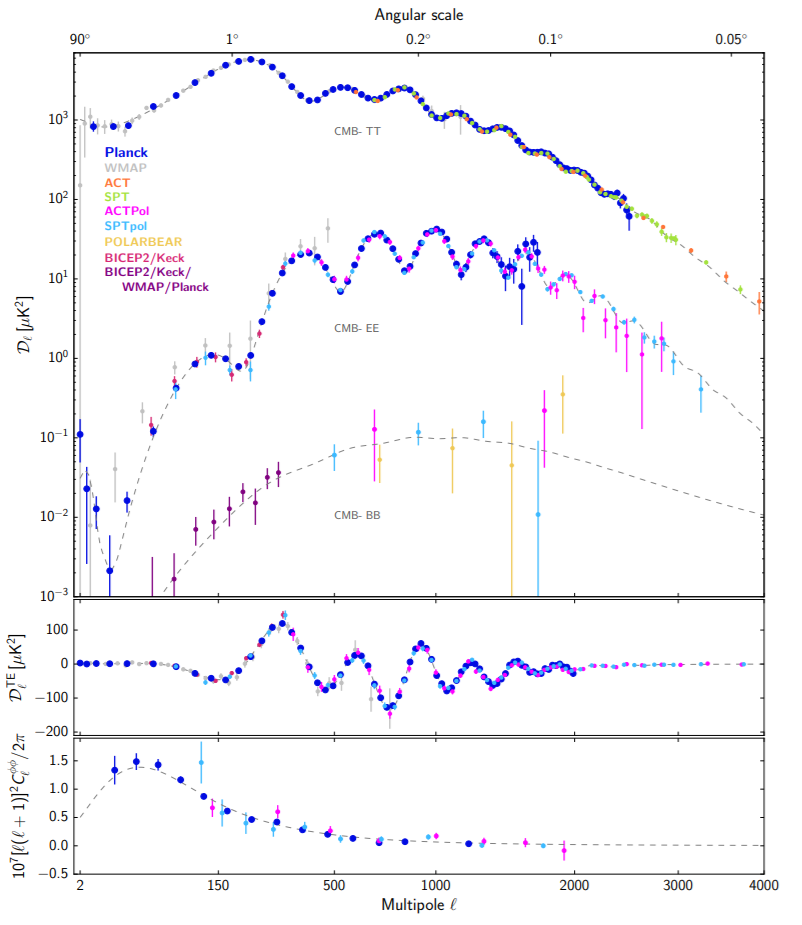
\includegraphics[width=0.85\textwidth]{cosmo_evol/CMB_compilation.png}
    \caption{Compilation of recent CMB angular power spectrum measurements from which most cosmological inferences are drawn.The upper panel shows the power spectra of the temperature and E-mode and B-mode polarization signals, the next panel the cross-correlation spectrum between T and E, while the lower panel shows the lensing deflection power spectrum. Different colours correspond to different experiments, each retaining its original binning. For Planck, ACTPol, and SPTpol, the EE points with large error bars are not plotted (to avoid clutter). The dashed line shows the best-fit \LCDM\ model to the Planck temperature, polarization, and lensing data. \textit{Note:} Reprinted from \textcite{2018arXiv180706205P}.}
    \label{fig:cmb_compilation}
\end{figure}
%%%%%%%%%%%%%%%%%%%%%%%
% Supernovae
%%%%%%%%%%%%%%%%%%%%%%%
\subsection{Supernovae}
Supernovae (SNe) are the most straightforward tool for studying cosmic acceleration, as they directly discovered the acceleration in the first place \parencite{riess}. Type Ia supernovae (SNe Ia) are exploding stars defined by the lack of hydrogen and the presence of silicon in their early-time spectra \parencite{SN}, and are a product of a thermonuclear explosion of a C/O white dwarf. Observations show that SNe Ia have a luminosity peak that is tightly correlated with the shape of their light curves -- supernovae that rise and fall more slowly have higher peak luminosity \parencite[first quantified by][]{SN_lum}. From observations of (multiband) light curve shapes and colors the luminosity at a brightness peak can be predicted.

To measure cosmic expansion with Type Ia SNe, the observed flux and predicted luminosity are compared. From that the supernova's luminosity distance can be measured. An accurate redshift is obtained by measuring the host galaxy (calibrator). Since the distances to the local calibrators are usually determined from the Hubble expansion, this method gives the luminosity distance $D_L$ in units of $h\mins$ Mpc. Measured relation is used to constraint dark energy parameters.

Recent analysis of \textcite{Abbott_2019} uses data from the Dark Energy Survey Supernova Program (DES-SN) -- 207 spectroscopically confirmed SNe Ia from the first three years of DES-SN combined with a low-redshift sample of 122 SNe from the literature. For a flat $w$CDM\ model they found a matter density $\Omega_m=0.321\pm0.018$ and an equation of state $w=-0.978\pm0.059$, see \autoref{fig:des_sne_results}.

\begin{figure}[hbt]
    \centering
    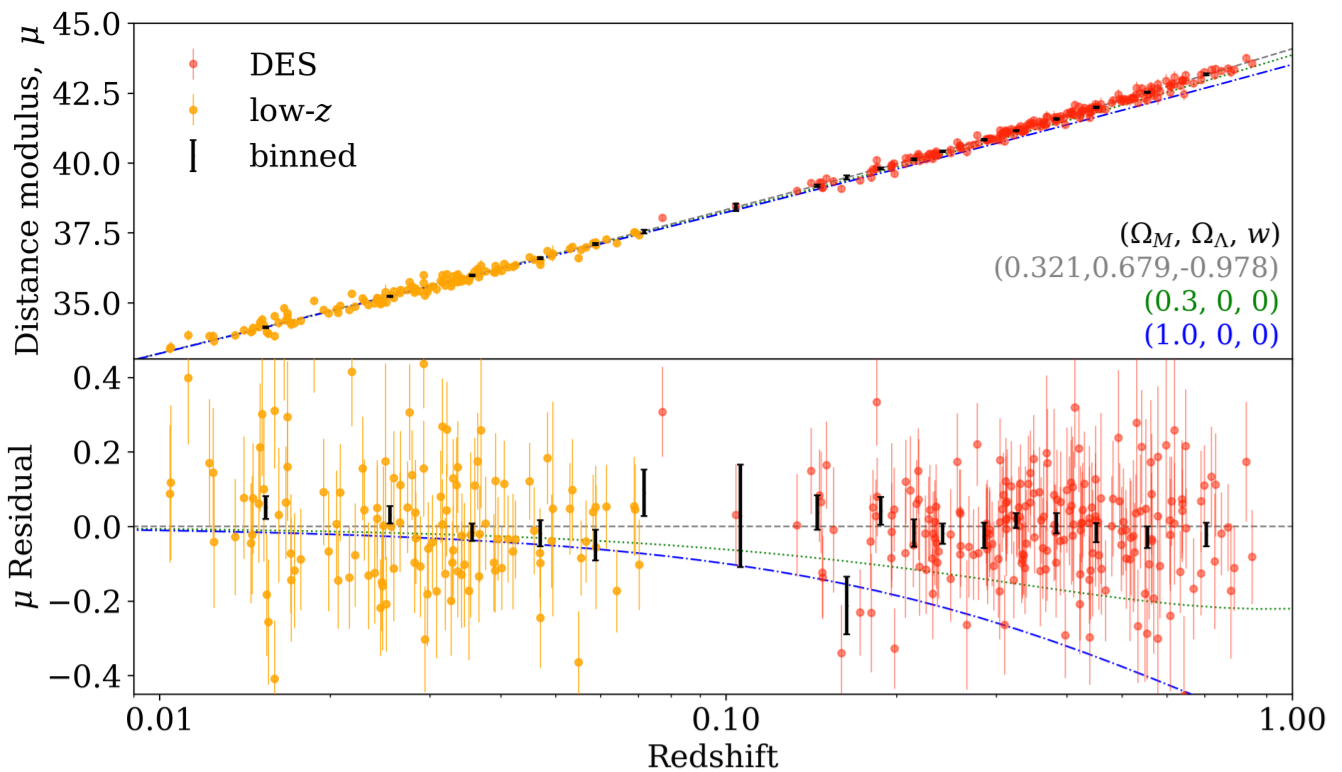
\includegraphics[width=0.7\textwidth]{cosmo_evol/DES_SNe_results.png}
    \caption{Hubble diagram for the DES-SN3YR sample. Top: distance modulus $(\mu =5\log [d_L/10\rm{pc}])$ from ``BEAMS with Bias Corrections'' fit \parencite{Kessler_2017}, black bars, which are used for cosmology fits) and for each SN (red, orange circles). The dashed gray line shows best fit model, while the green and blue dotted lines show models with no dark energy and matter densities $\Omega_m = 0.3$ and $1.0$ respectively. Bottom: residuals to the best fit model; $1\sigma$ error bars show 68\% confidence. \textit{Note:} Reprinted from \textcite{Abbott_2019}.}
    \label{fig:des_sne_results}
\end{figure}
%%%%%%%%%%%%%%%%%%%%%%%
% BAO
%%%%%%%%%%%%%%%%%%%%%%%
\subsection{Baryonic acoustic oscillations}
\label{sec:bao}
Baryonic acoustic oscillations (BAO) provide an entirely independent way of measuring cosmic distance. Sound waves propagating before recombination imprint a characteristic scale on matter clustering. The acoustic length scale can be computed as
\eq{
r_s=\int_0^{t_\ast}{\frac{c_s(t)}{a(t)}\dd t}=\int_{z_\ast}^{\infty}{\frac{c_s(z)}{H(z)}\dd z},
}
where asterisk denotes time (redshift) at recombination and $c_s$ is the sound speed. The behavior of $H(z)$ depends on the ratio of the matter density to radiation density and the sound speed depends on the ratio of radiation pressure to the energy density of the baryon-photon fluid, determined by the baryon-to-photon ratio. Both the matter-to-radiation ratio and the baryon-to-photon ratio can be measured from the CMB anisotropy power spectrum. This gives $r_s\sim150$ Mpc. The scale of the acoustic feature is stable to better than 1\% accuracy, making it an excellent standard ruler.

This effect can be detected in the angular clustering of galaxies in bins of photometric redshift, yielding the angular diameter distance. Furthermore, measuring the BAO scale in a velocity separation allows a direct determination of $H(z)$. The BAO method measures $D(z)$ in absolute units -- Mpc not $h\mins$ Mpc like SNe measurements, and thus BAO measurements to the same redshift carry different information. At low redshift $(z\lesssim0.5)$, the BAO method strongly complements SN measurements, while at higher redshift $(z\gtrsim0.5)$ the BAO method is an powerful probe of dark energy and cosmic geometry.

BAO can be clearly seen in the correlation function \parencite[see e.g.][]{1993ApJ...412...64L} for definition and estimators). The two-point correlation function $\xi(r)$ is the excess probability $\dd P$ of finding two pairs of galaxies in two volumes $\dd V_1$ and $\dd V_2$ at a given comoving distance $r$
\eq{
    \label{eq:corr}
    \dd P = \bar{n}^2[1+\xi(r)]\dd V_1 \dd V_2\,,
}
where $\bar{n}$ is the expected density of the distribution. The distances are usually measured using the redshift in the redshift space where the distortions (see \autoref{sec:rsd}) cause the redshift-space correlation $\xi(s)$ function to vary according to the angle between the separation vector and the line of sight. In \autoref{fig:xi_s} we see the spherically averaged correlation function from \textcite{2005ApJ...633..560E} with the clear bump at $100h^{-1}$ Mpc scale.
\begin{figure}[hbt]
    \centering
    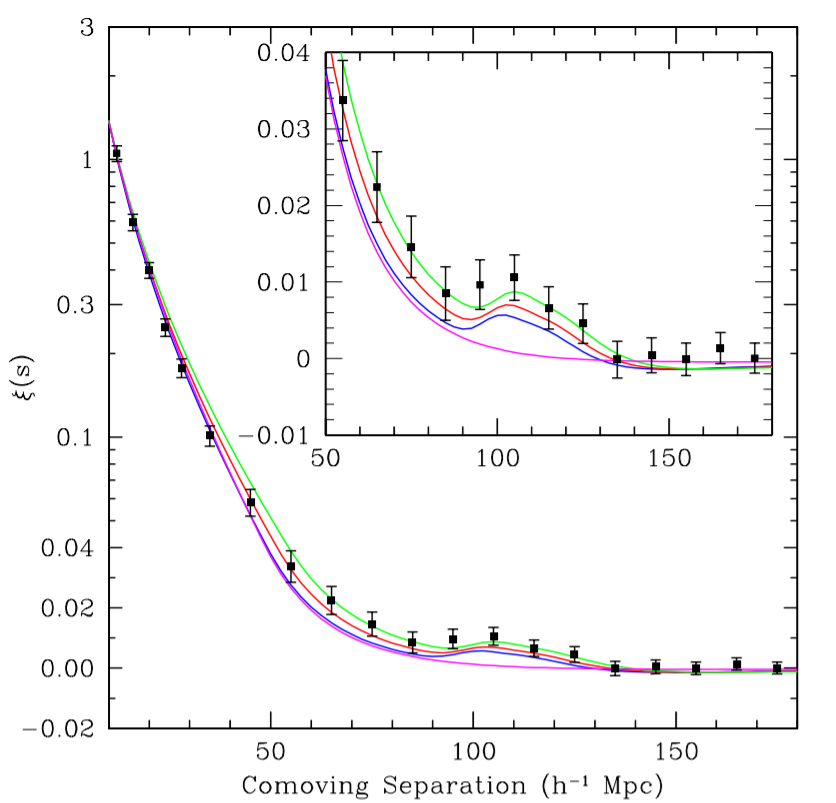
\includegraphics[width=0.7\textwidth]{cosmo_evol/bao_rsd.png}
    \caption{The large-scale redshift-space correlation function of the SDSS LRG sample. The error bars are from the diagonal elements of the mock-catalog covariance matrix; however, the points are correlated. Note that the vertical axis mixes logarithmic and linear scalings. The inset shows an expanded view with a linear vertical axis. The models are $\Omega_mh^2=0.12$ (top, green), $0.13$ (red), and $0.14$ (bottom with peak, blue), all with $\Omega_bh^2=0.024$ and $n=0.89$ and with a mild non-linear prescription folded in. The magenta line shows a pure CDM model ($\Omega_mh^2=0.105$), which lacks the acoustic peak. It is interesting to note that although the data appears higher than the models, the covariance between the points is soft as regards overall shifts in $\xi(s)$. Subtracting $0.002$ from $\xi(s)$ at all scales makes the plot look cosmetically perfect, but changes the best-fit $\chi^2$ by only $1.3$. The bump at$100h^{-1}$ Mpc scale, on the other hand, is statistically significant. \textit{Note:} Reprinted from \textcite{2005ApJ...633..560E}.}
    \label{fig:xi_s}
\end{figure}

In \textcite{BAO_results} present a measurement of the BAO from the three-dimensional correlation of Lyman-$\alpha$ forest absorption and quasars from the SDSS Data Release 14 (the first two years of observations by the eBOSS) at redshift $z=2.35$. The position of the BAO peak is used to determine the Hubble distance $d_H$ and the comoving angular diameter distance $d_A$ relative to the sound horizon at the drag epoch $r_s: d_H(z=2.35)/r_s = 9.20\pm0.36$ and $d_M(z=2.35)/r_s = 36.3\pm1.8$. These results are $1.5\sigma$ from the flat \LCDM\ model of \textcite{2016A&A...594A..13P}.
%%%%%%%%%%%%%%%%%%%%%%%
% WL
%%%%%%%%%%%%%%%%%%%%%%%
\subsection{Weak lensing}
Gravitational lensing is the deflection of light from distant sources due to the bending of space-time by baryonic and dark matter (lenses) along the line of sight. It is a very useful cosmological probe because it is sensitive to all matter regardless of its nature. In the limit of very small deflection angles it is called weak lensing (WL). WL causes tiny distortions ($\sim0.5\%$), or ``shear'', in galaxy sizes and shapes -- see \autoref{fig_WL_Abell}. Intrinsic size or shape of a given galaxy are unknown, but normally, galaxy orientations are assumed to be random ($\sim30\%$ dispersion), so they should not exhibit statistically significant and coherent alignments. In the presence of lensing, small but coherent shears in background galaxy images are induced. This means that WL is statistically detectable by averaging shapes over many lensed galaxies. In principle either the shearing of galaxies (shape distortion) or their magnification (size distortion) can be measured. However, in practice the shape distortions is used much more widely, since the scatter in shapes of galaxies is less than the scatter in their sizes.

% \todo{
% \subsubsection{Current Limits}
% Using the Shapiro time delay one can obtain strong limits on the \textit{gravitational slip} (combination $\Psi-\Phi$) in the solar system. The round-trip time of signals from the Cassini spacecraft near Saturn as the signals pass close to the sun is longer than one would expect in flat spacetime. This gives tight limit on the slip \parencite{test_pot_1}
% \eq{
%     \frac{|\Psi-\Phi|}{\Phi}=(2.1\pm2.3)\cdot\EXP{-5}
% }
% within the solar system. Combining stellar dynamics with the strong gravitational lensing on galaxy scales limit the slip \parencite{test_pot_2}
% \eq{
%     \frac{|\Psi-\Phi|}{\Phi}=0.01\pm0.05
% }
% on kpc scales. Future surveys such as the LSST and Euclid will improve these limits and provide new one on larger scales.
% }%% end TODO
Weak lensing provides a direct measure of the distribution of matter, independent of any assumptions about galaxy biasing. Since this distribution can be predicted theoretically, and its amplitude can be directly used to constrain cosmology, weak lensing has great potential as a cosmological probe. The correlation of the density field of nearby galaxies with the lensing shear measured on more distant galaxies is called \textit{galaxy-galaxy lensing}. Most lens systems involve sources (and lenses) at moderate or high redshift, and thus can lensing probe the geometry of the Universe -- the measurement of the shear correlation function as a function of the redshifts of observed galaxies is called \textit{tomography}. The scaling of the galaxy-galaxy lensing signal as a function of the source redshift, known as \textit{cosmography}, depends purely on geometric factors and hence can be used to construct a distance-redshift relation.
\begin{figure}
	\centering
		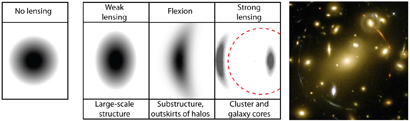
\includegraphics[scale=1.00]{cosmo_evol/WL_abel.jpg}
	\caption{(Left) Illustrations of the effect of a lensing mass on a circularly symmetric image. Weak lensing elliptically distorts the image, flexion provides an arc-ness and strong lensing creates large arcs and multiple images. (Right) Galaxy cluster Abell 2218, strongly lensed arcs can be seen in around the cluster. Every background galaxy is weakly lensed. \textit{Note:} From NASA, ESA, and Johan Richard (Caltech, USA).}
	\label{fig_WL_Abell}
\end{figure}
%%%%%%%%%%%%%%%%%%%%%%%
% Large-scale structure
%%%%%%%%%%%%%%%%%%%%%%%
\subsection{Large-scale structure}
Studying the large-scale structures (LSS) of the Universe is of a great importance for the cosmology. Since the clustering of matter on scales from galaxies to superclusters came from quantum fluctuations in the very early Universe with important modification by radiation and baryons, the LSS encode critical information about the contents of the Universe, the origin of the fluctuations, and the cosmic expansion background in which the structures evolved.

Measurements of large-scale power spectrum for the spatial distribution of matter as a function of redshift constrain the cosmic expansion history, the cosmological distance scale, the growth rate of structures, the mass of the neutrinos and the abundance of dark matter. This includes BAO measurement of the distance-redshift relation (as a standard ruler). The BAO with the growth of the LSS in the Universe form two robust probes of dark energy, and a potential discriminator between dark energy and modified gravity models. Beyond the dark energy, the large scale power spectrum is a probe of both neutrino mass and primordial non-gaussianity.
\subsubsection{Matter power spectrum}
The matter power spectrum $P(k)$ is defined as a quadratic function of the Fourier transformation of the density contrast $\delta$
\eq{
  \label{eq:pk}
  P(k)(2\pi)^3\delta_{\rm D}(k-k')\equiv \left\langle \hat\delta(k)\hat\delta^*(k')\right\rangle\,,
}
where $\delta_{\rm D}$ is the Dirac delta function and we are averaging over possible realizations. The power spectrum is by far the most common descriptor of clustering in the linear and mildly non-linear regime and plays a central role in cosmology. The power spectrum is the Fourier transform of the correlation function \eqref{eq:corr}
\eq{
    P(k)=\int\xi(r)e^{-ik\cdot r}\dd^3r\,.
}
However what we observe in practice is the galaxy density contrast $\delta_g$, which is different from the total matter density contrast $\delta_m$. The two quantities are assumed to be related by a bias factor $b$ defined by
\eq{
    b\equiv\frac{\delta_g}{\delta_m}\,,
}
from which follows $P_g(k)=b^2P_m(k)$. The idea of a simple biasing scheme tries to capture physics beyond the purely linear gravitational treatment, e.g. merging processes or evolutionary processes that render galaxies brighter or dimmer and therefore visible or invisible to our telescopes.

In \autoref{fig:pk_planck} is shown (linear) matter power spectrum inferred from different cosmological probes \parencite{2018arXiv180706205P}.
\begin{figure}[hbt]
    \centering
    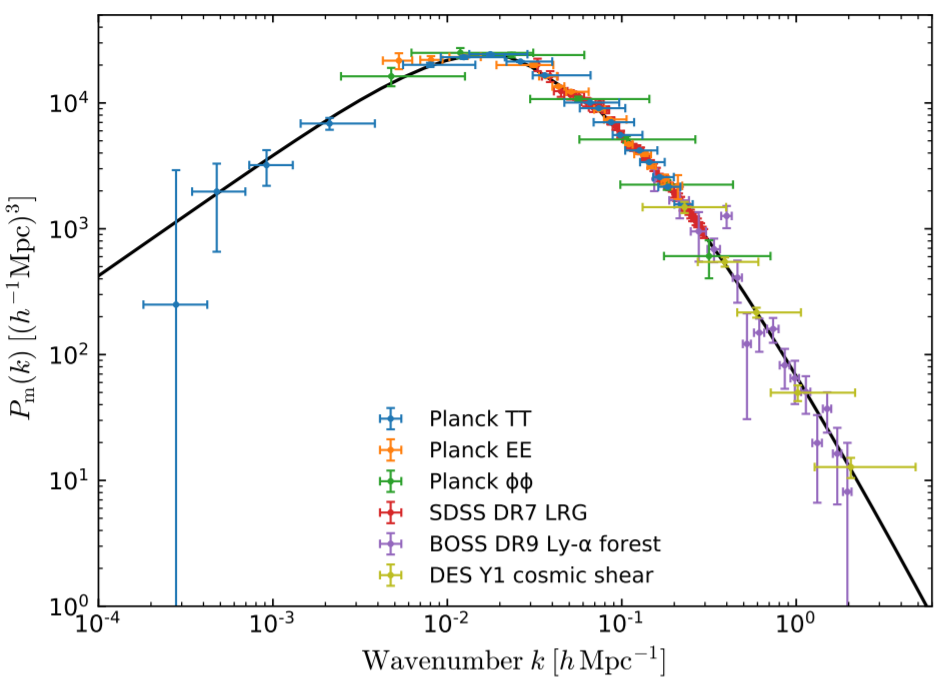
\includegraphics[width=0.7\textwidth]{cosmo_evol/pk_planck.png}
    \caption{The (linear theory) matter power spectrum (at z = 0) inferred from different cosmological probes. The broad agreement of the model (black line) with such a disparate compilation of data, spanning 14 Gyr in time and three decades in scale is an impressive testament to the explanatory power of \LCDM. Earlier versions of similar plots can be found in, for example, \textcite{1994ARA&A..32..319W}, \textcite{1995Sci...268..829S}, \textcite{2002PhRvD..66j3508T}, and \textcite{2004ApJ...606..702T}. A comparison with those papers shows that the evolution of the field in the last two decades has been dramatic, with \LCDM\ continuing to provide a good fit on these scales. \textit{Note:} Reprinted from \textcite{2018arXiv180706205P}.}
    \label{fig:pk_planck}
\end{figure}

%%%%%%%%%%%%%%%%%%%%%%%
% Galaxy clusters
%%%%%%%%%%%%%%%%%%%%%%%
\subsection{Galaxy clusters}
The observed number density and clustering of galaxy clusters as a function of mass and redshift provides a powerful toolset to constraining cosmology.  Galaxy clusters provided the first line of evidence for the existence of dark matter \textcite{zwicky} and cluster mass-to-light ratio measurements suggested that the matter density in the universe was sub-critical \textcite{Gott}. Galaxy clusters measurements are sensitive to both the expansion history and the growth of structure in the Universe enabling to distinguish between dark energy and modified gravity models for cosmic acceleration. Additional probes are measurements of the baryonic mass fraction in clusters, and of the tomographic lensing signatures through clusters.

The basic idea of cluster abundance studies is to compare the predicted space density of massive halos to the observed space density of clusters. The basic observables are the richness, the number of galaxies in a specified luminosity and color range. Halo abundance is sensitive to the amplitude of the matter power-spectrum $\sigma_8$ and the matter density $\Omega_m$, more precisely a combination of a form $\sigma_8\Omega_m^q$, with $q\approx0.4$ \textcite{white}. The degeneracy between $\sigma_8$ and $\Omega_m$ can be broken by measuring abundances at a variety of masses.
% \subsubsection{Spherical collapse}
% If we assume a spherical overdensity of pressureless matter in an expanding Universe we can arrive to the following equation \parencite{2010deto.book.....A}
% \eq{
%     \delta''+\left(1+\frac{\HH'}{\HH}\right)\delta'-\frac32\Omega_m\delta=\frac43\frac{\delta'^2}{1+\delta}+\frac32\Omega_m\delta^2\,,
% }
% which has a solution in the Einstein--de Sitter Universe
\subsubsection{The halo mass function}
The halo mass function $\dd n/\dd M$ is defined as the number of haloes of mass $M$ per unit volume per unit interval in $M$. To describe the halo mass function we need two other quantities, $f(\sigma)$ and $\ln\sigma^{-1}$. The rms linear overdensity $\sigma$ of the density field smoothed with a top-hat filter $W$ with a radius that encloses a mass $M$ at the mean cosmic matter density is defined as
\eq{
    \sigma^2(M, z)=\frac{D^2(z)}{2\pi^2}\int_0^\infty{k^2P(k)W^2(k,M)\dd k}\,.
}
The mass function is then written as
\eq{
    \dddd nM=\frac{\rho_0}{M}\dddd{\ln\sigma^{-1}}{M}f(\sigma)\,,
}
where all the cosmological information is contained in the function \(f(\sigma)\) --  the fraction of mass in collapsed haloes per unit interval in $\ln\sigma$. This function depends on how haloes are defined, usually using the friends-of-friends (FoF) algorithm of \textcite{1985ApJ...292..371D}. The analytical form of $f(\sigma)$ using the asumtpion of of collisionless spherical collapse has been proposed by \textcite{1974ApJ...187..425P}
\eq{
    f(\sigma) = \sqrt{\frac2\pi}\frac{\delta_c}{\sigma}\exp{\left(-\frac{\delta_c^2}{2\sigma^2}\right)}\,,
}
where the parameter \(\delta_c=1.686\) can be interpreted physically as the linearly extrapolated overdensity of a top-hat spherical density perturbation at the moment of maximum compression for an Einstein de-Sitter universe.
%%%%%%%%%%%%%%%%%%%%%%%
% Strong lensing
%%%%%%%%%%%%%%%%%%%%%%%
\subsection{Strong lensing}
Strong gravitational lensing (SL) refers to the multiple imaging of a background object due to a massive foreground object (typically clusters of galaxies) -- see \autoref{fig_WL_Abell}. The resulting angular displacement, morphological distortion, and time delay can be used to measure dark energy parameters. Strong gravitational lensing time delays measure a combination of distances that combining with other dark energy probes can further constraint cosmological parameters. The time delays is also expected to test gravity on scales where the screening mechanisms is becoming active.

Another independent way to measure dark energy parameters with SL is the analysis of systems with multiple sets of multiple images \textcite{SL_in_CLGs}. The positions of these multiple images depend strongly on the detailed properties of the lens mass distribution and on the angular diameter distance ratios between the lens, source and observer, they encapsulate information about the underlying cosmology. This dependence on the geometry can be used to derive constraints on the cosmological parameters.
%%%%%%%%%%%%%%%%%%%%%%%
% Redshift-space distortions
%%%%%%%%%%%%%%%%%%%%%%%
\subsection{Redshift-space distortions}
\label{sec:rsd}
When we observe distant galaxies, two features determine their redshifts -- the Hubble expansion and their peculiar velocities. The peculiar velocities of galaxies thus cause them to appear displaced along the line of sight in redshift space. These displacements lead to redshift distortions in the pattern of clustering of galaxies in redshift space and make large scale galaxy clustering anisotropic. Redshift-space distortions (RSD) have the tremendous advantage of bearing information about the dynamics of galaxies.

The coordinate transformation from real space $(r)$ to redshift space $(s)$ of a source with a peculiar velocity $\bm v$ is given by
\eq{
    \mb s = \mb r\left[1+\frac{u(r)-u(0)}{r}\right]\,,
}
whre $u\equiv\mb v\cdot\mb r/r$. The strength of the anisotropy is governed by distortion parameter $\beta = f(z)/b(z)$, where $f(z)$ is the logarithmic growth rate of fluctuations \eqref{eq:grw_rate} and $b$ is the bias. By modeling the full redshift-space galaxy power spectrum one can obtain combination of the product of the matter clustering amplitude and the growth rate.

Anisotropy of galaxy clustering offers an alternative to weak lensing and cluster abundances as a tool for measuring the growth of structures. RSD directly measure the rate at which structure is growing at the redshift of observation unlike WL and galaxy cluster measurements  which measure the rate of growth at multiple redshifts. RSD measurements can improve constraints on dark energy models and they can be used to constrain departures from GR by testing consistency of the growth and expansion histories. The key challenge in modeling RSD is accounting for nonlinear effects, including nonlinear or scale-dependent bias between galaxies and matter, at the level of accuracy demanded by the LSST`s precision.


%%%%%%%%%%%%%%%%%%%%%%%
% Standard LCDM model
%%%%%%%%%%%%%%%%%%%%%%%
\section{Standard \LCDM\ model -- successes and issues}
Standard cosmological model, the \LCDM\ model or the concordance model, assumes that the Universe was created in the Big Bang from infinitely hot and dense energy and now is the Universe composed of about 5\% ordinary matter, 27\% dark matter, and 68\% dark energy \parencite{redefineLCDM}. The \LCDM\ model is based upon two theoretical models -- the Standard Model of Particle Physics and  the General Theory of Relativity. The model also assumes that the universe is homogeneous and isotropic on sufficiently large (cosmic) scales. The model is mathematically described above in \autoref{chpt:cosmo_evol}.

The \LCDM\ model represents general relativity with a cosmological constant \(\Lambda\) which is associated with dark energy and a universe containing sufficiently massive dark matter particles, i.e., cold dark matter. However, the nature of both dark energy and dark matter is unknown.

In 1948, \textcite{PhysRev.74.505.2} suggested that the elements could have been made during the early hot matter-energy phase associated with the Big Bang and predicted their representation -- hydrogen about 75\%, helium about 25\% and small amounts of deuterium, lithium, and other light elements.

The other great success of the Big bang model is prediction of the Cosmic Microwave Background (CMB) radiation and its temperature. In 1948, \textcite{1948Natur.162..774A} calculated the present temperature of the CMB to be about 5 K, remarkably close to the modern value of about 2.73 K, determined by the COBE satellite. In addition, the COBE results showed an extremely isotropic and homogeneous CMB. This led to the need for an inflationary phase \parencite{1981PhRvD..23..347G} of strongly accelerated expansion prior to the decoupling of photons from ordinary matter.

The \LCDM\ model has an additional major assumption about existence of dark matter. The notion of dark matter arose from observations of large astronomical objects such as galaxies and clusters of galaxies, which displayed gravitational effects that could not be accounted for by the visible matter. In particular, the observations of \textcite{1980ApJ...238..471R}, who measured the rotation curves for the luminous matter of many spiral galaxies together with the observations of \textcite{1978PhDT.......195B}, who compiled 21 cm rotation curves for neutral hydrogen gas that extended far beyond the luminous matter of each galaxy, showed that the composite rotation curves were essentially flat out to the edge of the 21 cm data. This implied that considerably more mass was required to be present in each galaxy. This invisible matter was called dark matter and since to date no dark matter has been definitely detected and the nature of dark matter remains unknown.

The notion of dark energy arose from two sets of observations of supernovae of Type Ia by \textcite{riess} and \textcite{1999ApJ...517..565P} that suggested that the expansion of the universe is accelerating. The conclusion from these observations was that the universe had to contain enough energy to overcome gravity. This energy was named “dark energy.”

\subsection{Cosmological constant problem}
\label{ssec:lambda}
Standard cosmological \LCDM\ model described above is in a good agreement with all measurements of CMB \parencite{planck_cosm}, type Ia supernovae \parencite{Abbott_2019}, or BAO \parencite{BAO_results}. However, this concordance model, and namely the cosmological constant, has some significant fundamental problems. Usually, the fine-tuning of the cosmological constant is presented as the main issue but the real issue with the cosmological constant is radiative instability, and the need to \textbf{repeatedly} fine tune whenever the higher loop corrections are included. We will describe here only the main idea behind these problems, for more detailed overview see e.g. \textcite{2015arXiv150205296P,2012CRPhy..13..566M}.

The action of the general relativity, together with the action describing matter, is
\eq{
	\label{eq:S_GR}
	S=\frac{\Mpl^2}{2}\int\dd^4x\dg\left(R-2\Lambda_B\right)+S_m[\psi_m;g_\uv]\,,
}
where $\Mpl\equiv(\sqrt{8\pi G})^{-1}$ is the reduced Planck mass, $R$ is the Ricci scalar (curvature), $\Lambda_B$ the bare cosmological constant and $S_m[\psi_m;g_\uv]$ represents the action of matter fields. The first term $(R)$ is the standard Einstein-Hilbert action. The \textit{bare} cosmological constant appears in the second term of the above expression and it is merely a new parameter of the total action. As it is compatible with general covariance this term appears to be totally natural from the relativistic point of view. The third term in the above equation denotes the generic matter action. Variation of the total action with respect to the metric tensor leads to the Einstein equations of motion
\eq{
    R_\uv-\frac12Rg_\uv+\Lambda_Bg_\uv=\frac{1}{\Mpl^2}T_\uv\,,
}
where the stress-energy tensor is defined by
\eq{
    T_\uv=-\frac{2}{\dg}\frac{\delta S_m}{\delta g^\uv}\,.
}
As shown by \textcite{1968SPhD...12.1040S}, when one takes into an account quantum field theory the picture is changed. The stress energy tensor of a field placed in the vacuum state is given by
\eq{
    \left\langle0\left|T_\uv\right|0\right\rangle=-\rho\vac g_\uv\,,
}
where $\rho\vac$ is the constant energy density of the vacuum. The vacuum fluctuations are just a specific type of energy and, in general relativity, all forms of energy gravitate. Therefore, the Einstein equations when quantum field theory is taken into account are
\eq{
    R_\uv-\frac12Rg_\uv+\Lambda\eff g_\uv=\frac{1}{\Mpl^2}T_\uv\,,
}
where
\eq{
    \Lambda\eff=\Lambda_B+\frac{1}{\Mpl^2}\rho\vac\,.
}
Therefore, we conclude that the effective cosmological constant is the sum of the bare cosmological constant and of a contribution originating from the vacuum fluctuations. The effective cosmological constant $\Lambda\eff$ is the quantity that one can observe and constrain when tests of the Einstein equations are carried out. The problem is that $\rho\vac$ is made of several terms which are all huge in comparison with the observed value of $\Lambda\eff$ and need to be fine-tunned.
\subsubsection{Phase Transitions}
\begin{sloppypar}
Another problem with fine-tuning of the cosmological constant comes from changes in the vacuum energy during phase transitions such as was the electro-weak phase transition. The contribution to the vacuum energy coming from the minimum of a potential of some field, in this case the Higgs field, changes as the field takes its new position after the transition. One can calculate this contribution \parencite{2012CRPhy..13..566M} and for the the mass of the Higgs boson $m_H=125$ GeV arrives at
\end{sloppypar}
\eq{
    \rho\vac^{EW}\simeq -10^{55}\rho\crit\,.
}
For the quantum chromo-dynamics transition, one can compute
\eq{
    \rho\vac^{EW}\simeq10^{45}\rho\crit\,.
}
If we fine-tune the vacuum energy to be zero today it had to be non-zero (and huge) before each of these transitions.
\subsubsection{Zero-Point Energy Density}
When we consider a simple real free scalar field with the potential $V(\Phi)=2m^2\Phi^2/2)$ we will arrive at the vacuum energy
\eq{
    \left\langle \rho \right\rangle = \left\langle0\left|T_{00}\right|0\right\rangle=\frac{1}{2\pi^3}\frac12\int\dd^3k\sqrt{k^2+m^2}\,.
}
This contribution to the cosmological constant blows up in the ultra-violet regime and is infinite. But this is nothing new in the quantum field theory. If we apply the dimensional regularization \parencite{tHooft:1972tcz} and subtract the pole as usual, one is left with finite energy density of the vacuum
\eq{
    \left\langle \rho \right\rangle = \frac{m^4}{64\pi^2}\ln{\left(\frac{m^2}{\mu^2}\right)}\,,
}
where $\mu$ is a regularization scale. We see that the contribution is proportional to the fourth power of the mass of the particle and therefore, e.g., the photon does not contribute to the vacuum energy density. The equation was derived for free scalar field but similar contributions with different pre-factors can be computed for all other fields. The overal vacuum energy density is then
\eq{
    \label{eq:vac_all}
    \rho\vac=\sum_in_i\frac{m_i^4}{64\pi^4}\ln{\left(\frac{m_i^2}{\mu^2}\right)} + \rho_B + \rho\vac^{EW} + \rho\vac^{QCD}\,,
}
where $n_H=1$ for the Higgs boson, $n_f=4$ for fermions and $n_V=3$ for massive vector fields. For the renormalization scale $\mu\simeq3\times10^{-25}$, as discussed in \textcite{2011arXiv1105.6296K}, one calculates the contribution from the zero-point energy of particles to be  $\rho\vac\simeq-2\times10^8$ GeV$^4$
\subsubsection{Radiative instability}
The one loop contributions \eqref{eq:vac_all} to the vacuum energy can be fine-tunned via the bare cosmological constant and associated $\rho_B$. Even though the cancellation has to be very precise (one part in $\sim10^{60}$) we can be fine with this solution. Problems come with two-loops correction which is not significantly suppressed with respect to the one loop contribution \todo{CITE}. Therefore, the cancellation imposed at one loop is completely spoilt, and one must retune the finite contributions in the counterterm to more or less the same degree of accuracy. If we go further, to the three loops, four loops, and so on, we are required to fine tune each time to an extreme accuracy. This is radiative instability and main cosmological constant problem.

